\chapter{Thử nghiệm hệ thống}
\renewcommand{\baselinestretch}{1.2}
%\newcommand{\blank}[1]{\hspace*{#1}\linebreak[0]}
\section{Thử nghiệm tính ngữ nghĩa của câu truy vấn}
Để chứng minh tính đúng đắn của hệ thống, tôi thực hiện thử nghiệm hệ thống với một câu truy vấn: Liệt kê các thiết bị trong trung tâm HPCC. \\
Câu truy vấn tương ứng trong hệ thống của tôi là:
\myexample{Câu truy vấn tương ứng trong hệ thống}{
\{\\
\blank{1cm}"select" : "Source",\\
\blank{1cm}"where" : \{\\
\blank{2cm}"condition" : \{\\
\blank{3cm}"compare" : \{\\
\blank{4cm}    "keyword" : "SmartContextName",\\
\blank{4cm}    "comparator" : "=",\\
\blank{4cm}    "expression" : "HPCC"\\
\blank{3cm}\},\\
\blank{3cm}"logic" : \{\},\\
\blank{3cm}"in\_bracket" : \{\}\\
\blank{2cm}\}\\
\blank{1cm}\}\\
\}
}

Cơ chế truy vấn ngữ nghĩa: \\
\begin{figure}
	\center
	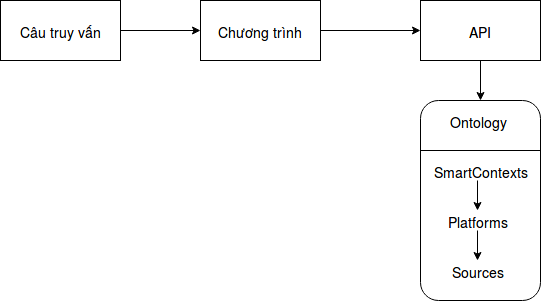
\includegraphics[scale=0.6]{image/demo}
	\caption{Cơ chế truy vấn ngữ nghĩa}
\end{figure}
Khi nhận được một câu truy vấn, hệ thống sẽ kiểm tra cú pháp câu truy vấn đó. Nếu cú pháp chính xác, sẽ gọi các API để trả về kết quả. Các API được xây dựng dựa trên mối quan hệ giữa các khái niệm trong ontology. Cụ thể trong trường hợp này, để trả về kết quả câu truy vấn, ta cần thực hiện các bước sau: \\
Đầu tiên, hệ thống sẽ tìm các SmartContext có tên là HPCC, kết quả thu được: \\
\myexample{}{
[\\
\blank{1cm}\{\\
\blank{2cm}'HasPlatform':[ ],\\
\blank{2cm}'ParentSmartContextId':[\\
\blank{3cm}'phong\_sinh\_vien\_id', \\
\blank{3cm}'phong\_can\_bo\_id', \\
\blank{3cm}'phong\_may\_chu\_id'\\
\blank{2cm}],\\
\blank{2cm}'SubSmartContextId':[ ],\\
\blank{2cm}'SmartContextId':'HPCC\_id',\\
\blank{2cm}'SmartContextName':'HPCC'\\
\blank{1cm}\}\\
]
}

Với mỗi SmartContext thu được, liệt kê các platform có trong đó: \\

\myexample{}{
[\\
\blank{1cm}\{\\
\blank{2cm}'PlatformHost':'http://192.168.0.197',\\
\blank{2cm}'PlatformId':'2667a8d0-0ff1-4d22-9153-26795502efc9',\\
\blank{2cm}'PlatformType':'',\\
\blank{2cm}'PlatformName':'openhab',\\
\blank{2cm}'PlatformPort':'8080',\\
\blank{2cm}'HasSource':[\\
\blank{3cm}'temperature-humidity-light\_openhab',\\
\blank{3cm}'motion\_openhab'\\
\blank{2cm}],\\
\blank{2cm}'PlatformStatus':'active'\\
\blank{1cm}\},\\
\blank{1cm}\{\\
\blank{2cm}'PlatformHost':'http://192.168.0.198',\\
\blank{2cm}'PlatformId':'0bafb5bf-5c16-4122-9782-d240914705d3',\\
\blank{2cm}'PlatformType':'',\\
\blank{2cm}'PlatformName':'thingsboard',\\
\blank{2cm}'PlatformPort':'8080',\\
\blank{2cm}'HasSource':[\\
\blank{3cm}'temperature-humidity-light\_thingsboard',\\
\blank{3cm}'motion\_thingsboard'\\
\blank{2cm}],\\
\blank{2cm}'PlatformStatus':'active'\\
\blank{1cm}\},
}
\myexample{}{
\blank{1cm}\{\\
\blank{2cm}'PlatformHost':'http://192.168.0.199',\\
\blank{2cm}'PlatformId':'611dc2c1-086d-487f-b44a-2d819764603a',\\
\blank{2cm}'PlatformType':'HomeAssistant',\\
\blank{2cm}'PlatformName':'homeassistant',\\
%}
%\myexample{}{
\blank{2cm}'PlatformPort':'8123',\\
\blank{2cm}'HasSource':[\\
\blank{3cm}'temperature-humidity-light\_homeassistant',\\
\blank{3cm}'motion\_homeassistant'\\
\blank{2cm}],\\
\blank{2cm}'PlatformStatus':'active'\\
\blank{1cm}\}\\
]
}

Ứng với mỗi platform, tìm các Soruce của mỗi platform. Ví dụ với platform OpenHAB:\\
\myexample{}{
[\\
\blank{1cm}\{\\
\blank{2cm}'LocalId':'temperature-humidity-light\_id',\\
\blank{2cm}'Label':'sensor',\\
\blank{2cm}'Description':'',\\
\blank{2cm}'SourceId':'temperature-humidity-light\_openhab',\\
\blank{2cm}'HasMetric':[\\
\blank{3cm}'Humidity',\\
\blank{3cm}'Temperature',\\
\blank{3cm}'Light'\\
\blank{2cm}],\\
\blank{2cm}'SourceType':'thing',\\
\blank{2cm}'SourceStatus':'active',
}
\myexample{}{
\blank{2cm}'EndPoint':'http://192.168.0.197:8080/source'\\
\blank{1cm}\},\\
\blank{1cm}\{\\
\blank{2cm}'LocalId':'motion\_id',\\
\blank{2cm}'Label':'sensor',\\
\blank{2cm}'Description':'',\\
\blank{2cm}'SourceId':'motion\_openhab',\\
\blank{2cm}'HasMetric':[\\
\blank{3cm}'LedDo',\\
\blank{3cm}'LedXanh',\\
\blank{3cm}'LedVang',\\
\blank{3cm}'Motion'\\
\blank{2cm}],\\
\blank{2cm}'SourceType':'thing',\\
\blank{2cm}'SourceStatus':'active',\\
\blank{2cm}'EndPoint':'http://192.168.0.197:8080/source'\\
\blank{1cm}\}\\
]
}

Kết quả cuối cùng thu được các Source của một SmartContext: \\

\myexample{}{
[\\
\blank{1cm}\{\\
\blank{2cm}'LocalId':'temperature-humidity-light\_id',\\
\blank{2cm}'SourceStatus':'active',\\
\blank{2cm}'Description':'',\\
\blank{2cm}'EndPoint':'http://192.168.0.197:8080/source',\\
\blank{2cm}'SourceId':'temperature-humidity-light\_openhab',
}
\myexample{}{
\blank{2cm}'HasMetric':[\\
\blank{3cm}'Humidity',\\
\blank{3cm}'Temperature',\\
\blank{3cm}'Light'\\
\blank{2cm}],\\
\blank{2cm}'SourceType':'thing',\\
\blank{2cm}'Label':'sensor'\\
\blank{1cm}\},\\
\blank{1cm}\{\\
\blank{2cm}'LocalId':'motion\_id',\\
\blank{2cm}'SourceStatus':'active',\\
\blank{2cm}'Description':'',\\
\blank{2cm}'EndPoint':'http://192.168.0.197:8080/source',\\
\blank{2cm}'SourceId':'motion\_openhab',\\
\blank{2cm}'HasMetric':[\\
\blank{3cm}'LedDo',\\
\blank{3cm}'LedXanh',\\
\blank{3cm}'LedVang',\\
\blank{3cm}'Motion'\\
\blank{2cm}],\\
\blank{2cm}'SourceType':'thing',\\
\blank{2cm}'Label':'sensor'\\
\blank{1cm}\},\\
\blank{1cm}\{\\
\blank{2cm}'LocalId':'temperature-humidity-light\_id',\\
\blank{2cm}'SourceStatus':'active',\\
\blank{2cm}'Description':'',\\
\blank{2cm}'EndPoint':'http://192.168.0.198:8080/source',\\
\blank{2cm}'SourceId':'temperature-humidity-light\_thingsboard',
}
\myexample{}{
\blank{2cm}'HasMetric':[\\
\blank{3cm}'b37a79a0-755c-11e9-abce-5bf295b292b2-light',\\
\blank{3cm}'b37a79a0-755c-11e9-abce-5bf295b292b2-temperature',\\
\blank{3cm}'b37a79a0-755c-11e9-abce-5bf295b292b2-humidity'\\
\blank{2cm}],\\
\blank{2cm}'SourceType':'thing',\\
\blank{2cm}'Label':'sensor'\\
\blank{1cm}\},\\
\blank{2cm}...\\
]
}
\clearpage

\section{Thử nghiệm tính mở rộng của hệ thống}
Để chứng minh hệ thống có tính khả mở, tôi thêm một nền tảng IoT là ThingsBoard vào hệ thống bằng việc viết thêm một driver để ánh xạ dữ liệu từ định dạng của ThingsBoard về định dạng của ontology. Tôi sẽ thực hiện câu truy vấn: Lấy tất cả các platform có trong trung tâm HPCC để chứng minh đã thêm được ThingsBoard vào hệ thống. \\
Câu truy vấn tương ứng trong hệ thống là:
%\begin{figure}
%	\center
%	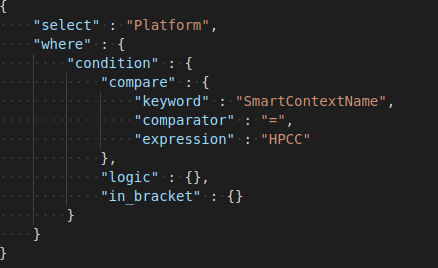
\includegraphics[scale=0.5]{image/add_thingsboard}
%	\caption{Thêm ThingsBoard vào hệ thống}
%\end{figure}
\myexample{Câu truy vấn tương ứng trong hệ thống}{
\{\\
\blank{1cm}"select" : "Platform",\\
\blank{1cm}"where" : \{\\
\blank{2cm}"condition" : \{\\
\blank{3cm}"compare" : \{\\
\blank{4cm}    "keyword" : "SmartContextName",\\
\blank{4cm}    "comparator" : "=",\\
\blank{4cm}    "expression" : "HPCC"\\
\blank{3cm}\},\\
\blank{3cm}"logic" : \{\},\\
\blank{3cm}"in\_bracket" : \{\}\\
\blank{2cm}\}\\
\blank{1cm}\}\\
\}\\
}

\clearpage
Kết quả thu được trước khi thêm Thingsboard, hệ thống chỉ có 2 nền tảng IoT: \\

\myexample{}{
[\\
\blank{1cm}\{\\
\blank{2cm}'PlatformId':'2667a8d0-0ff1-4d22-9153-26795502efc9',\\
\blank{2cm}'PlatformHost':'http://192.168.0.197',\\
\blank{2cm}'PlatformName':'openhab',\\
\blank{2cm}'HasSource':[\\
\blank{3cm}'temperature-humidity-light\_openhab',\\
\blank{3cm}'motion\_openhab'\\
\blank{2cm}],\\
\blank{2cm}'PlatformType':'',\\
\blank{2cm}'PlatformPort':'8080',\\
\blank{2cm}'PlatformStatus':'active'\\
\blank{1cm}\},\\
\blank{1cm}\{\\
\blank{2cm}'PlatformId':'611dc2c1-086d-487f-b44a-2d819764603a',\\
\blank{2cm}'PlatformHost':'http://192.168.0.199',\\
\blank{2cm}'PlatformName':'homeassistant',\\
\blank{2cm}'HasSource':[\\
\blank{3cm}'temperature-humidity-light\_homeassistant',\\
\blank{3cm}'motion\_homeassistant'
\blank{2cm}],\\
\blank{2cm}'PlatformType':'HomeAssistant',\\
\blank{2cm}'PlatformPort':'8123',\\
\blank{2cm}'PlatformStatus':'active'\\
\blank{1cm}\}\\
]
}
\clearpage
Kết quả thu được sau khi thêm Thingsboard, hệ thống có 3 nền tảng IoT:\\
\myexample{}{
[\\
\blank{1cm}\{\\
\blank{2cm}'PlatformId':'2667a8d0-0ff1-4d22-9153-26795502efc9',\\
\blank{2cm}'PlatformHost':'http://192.168.0.197',\\
\blank{2cm}'PlatformName':'openhab',\\
\blank{2cm}'HasSource':[\\
\blank{3cm}'temperature-humidity-light\_openhab',\\
\blank{3cm}'motion\_openhab'\\
\blank{2cm}],\\
\blank{2cm}'PlatformType':'',\\
\blank{2cm}'PlatformPort':'8080',\\
\blank{2cm}'PlatformStatus':'active'\\
\blank{1cm}\},\\
\blank{1cm}\{\\
\blank{2cm}'PlatformId':'0bafb5bf-5c16-4122-9782-d240914705d3',\\
\blank{2cm}'PlatformHost':'http://192.168.0.198',\\
\blank{2cm}'PlatformName':'thingsboard',\\
\blank{2cm}'HasSource':[\\
\blank{3cm}'temperature-humidity-light\_thingsboard',\\
\blank{3cm}'motion\_thingsboard'\\
\blank{2cm}],\\
\blank{2cm}'PlatformType':'',\\
\blank{2cm}'PlatformPort':'8080',\\
\blank{2cm}'PlatformStatus':'active'\\
\blank{1cm}\},\\
\blank{1cm}\{\\
\blank{2cm}'PlatformId':'611dc2c1-086d-487f-b44a-2d819764603a',
}
\myexample{}{
\blank{2cm}'PlatformHost':'http://192.168.0.199',\\
\blank{2cm}'PlatformName':'homeassistant',\\
\blank{2cm}'HasSource':[\\
\blank{3cm}'temperature-humidity-light\_homeassistant',\\
\blank{3cm}'motion\_homeassistant'\\
\blank{2cm}],\\
\blank{2cm}'PlatformType':'HomeAssistant',\\
\blank{2cm}'PlatformPort':'8123',\\
\blank{2cm}'PlatformStatus':'active'\\
\blank{1cm}\}\\
]
}


